\documentclass[12pt, a4paper]{article}
\usepackage[utf8]{inputenc}
\usepackage{appendix}
\usepackage{graphicx}
\usepackage{enumerate}
\usepackage{subfig}
\usepackage{float}
\usepackage{indentfirst}
\usepackage{amsmath}
\usepackage{amsfonts}
\usepackage{geometry}   %设置页边距的宏包
\usepackage{titlesec}   %设置页眉页脚的宏包
\usepackage{enumitem}
\usepackage{booktabs}
\usepackage{subfigure}
\usepackage[section]{placeins}
\geometry{left=2.54cm,right=2.54cm,top=2.54cm,bottom=2.54cm}


\begin{document}

\pagestyle{plain}

\begin{titlepage}

	\begin{center}	
	% Title

	\vspace{10ex}

	\hrule

	\vspace{2ex}

	\textbf{\Large{UM-SJTU} \Large{J}\large{oint} \Large{I}\large{nstitute} \\
	\Large{P}\large{HYSICS} \Large{L}\large{ABORATORY} \\
	\large{(}\Large{V}\large{P241)}}\\
	
	\vspace{2ex}

	\hrule
	
	\vspace{25ex}
	
	\Large{L}\large{ABORATORY} \Large{R}\large{EPORT}

	\vspace{6ex}

	\large{E}\normalsize{XERCISE 2}

	\vspace{4ex}

	% lab name here
	\large The Hall Probe: Characteristics and Applications

	\vspace{4ex}

	% group member here
	\begin{center}
		\begin{tabular}{lll}
		Name: Zhang Jiache & ID: 520370910044 & Group: 9
		\end{tabular}
	\end{center}

	% Bottom of the page
	{\large Date: \today}
	
	\end{center}
	
\end{titlepage}

\newpage

\section{Introduction}
This lab is designed to study and verify the principle and effects of Hall effect. Also we will learn the applications of Hall effect 
using a Hall probe. In detail, it is verifying that the Hall voltage is proportional to the magnetic field. What's more, we will calculate 
the magnetic field at the center of a solenoid, to find the sensitivity of an integrated Hall probe. The magnetic field distribution along 
the axis of the solenoid will be measured and compared with the corresponding theoretical curve.


\section{Theoretical Background}
\subsection{Hall Effect}
When we put a conducting sheet in a magnetic field, that the direction of the magnetic field \textbf{B} is perpendicular to the sheet, and 
let a electric current \textbf{I} passes through the sheet, we can observe a electric potential difference between the 
sides a and b of the sheet. The directon of electric field is both perpendicular to the current and the directio of the magnetic field. 
This is called the Hall effect, and the electric potential difference is Hall voltage $U_H$.
\begin{figure}[H]
	\centering
	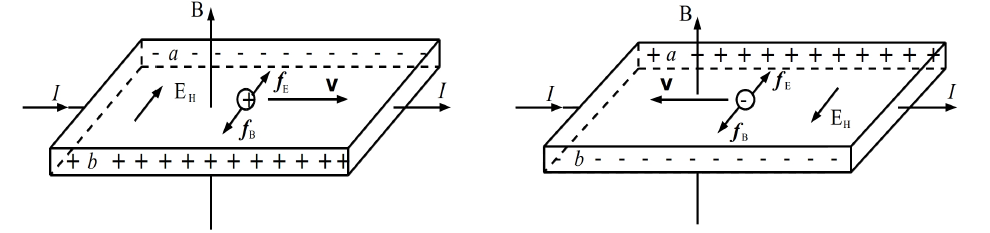
\includegraphics[scale = 0.6]{p1.png}
	\caption{The principle of Hall effect}	
\end{figure}

The Hall effect is caused by Lorenz force. When the charges move in the magnetic field, the Lorenz force $F_B$ leads to the deflection of 
the moving charges, so that they accumulate on one side of the sheet. The accumulated elctron results in a transverse electric field $E_H$ 
(The Hall field). Both electric force $F_E$ and the Lorenz force $F_B$ acts on the charges, and finally the two opposite forces will come to 
a balance when $U_H$  is stable. When the external magnetic field is not too strong, the Hall voltage is proportional to both the current and 
the magnitude of the magnetic field, and inversely proportional to the thickness of the sheet $d$:
\begin{equation}
	U_H = R_H \frac{IB}{d} = KIB
\end{equation}
Where $R_H$ is Hall coefficient and $K = R_H/d = K_H/I$, where $K_H$ is the sensitivity of the Hall element.

\subsection{Integrated Hall Probe}
When the sensitivity $K_H$ and current $I$ of a Hall probe are fixed, 
we can find the magnitude of the magnetic field by measuring the Hall 
voltage. We need to amplify the Hall voltage before measuring since it is usually very small.
\\ \newline
The following picture is a SS495A integrated Hall probe, which consists of a Hall sensor, an amplifier and a voltage compensator. 
The output voltage U can be read ignoring the residual voltage. The working voltage US = 5 V, and the output voltage U0 is 
approximately 2.5 V when the magnetic field is zero. The relation between the output voltage U and the magnitude
of the magnetic field is:
\begin{equation}
	B = \frac{U-U_0}{K_H}
\end{equation}
\begin{figure}[H]
	\centering
	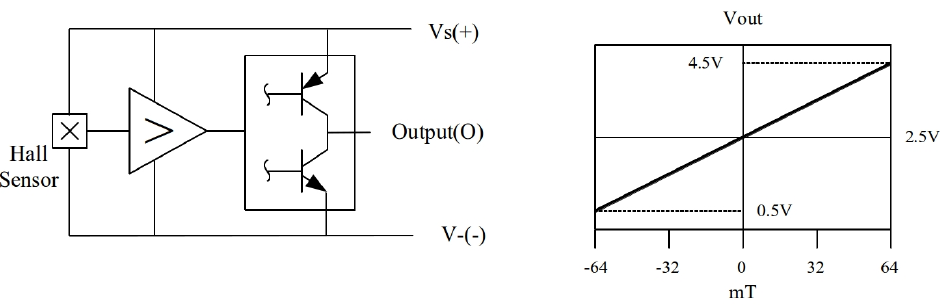
\includegraphics[scale = 0.6]{p2.png}
	\caption{The integrated Hall probe SS495A (left). The relation between the output
	voltage U and the magnitude of the magnetic field B (right).}
\end{figure}

\subsection{Magnetic Field Distribution Inside a Solenoid}
The magnetic field distribution on the axis of a single layer solenoid can be calculated
from the following formula:
\begin{equation}
	B(x)=\mu_0\dfrac{N}{L}I_M\begin{Bmatrix}
		\dfrac{L+2x}{2[D^2+(L+2x)^2]^{\frac{1}{2}}}+\dfrac{L-2x}{2[D^2+(L-2x)^2]^{\frac{1}{2}}}
		\end{Bmatrix}=C(x)I_M
\end{equation}
where $N$ is the number of turns of the solenoid, $L$ is its length, $I_M$ is the current through
the solenoid wire, and $D$ is the solenoid’s diameter. The magnetic permeability of vacuum
is $\mu_0 = 4\pi \times 10^{-7} H/m$.



\section{Experimental setup and Measurement procedure}
\subsection{Apparatus}
The experimental setup shown below consists of an integrated Hall probe SS495A
with $ K_H = 31.25 \pm 1.25 V/T $ or $ K_H = 3.125 \pm 0.125 mV/G $, 
a solenoid, a power supply, a voltmeter, a DC voltage divider, and a set of 
connecting wires.
\begin{figure}[H]
	\centering
	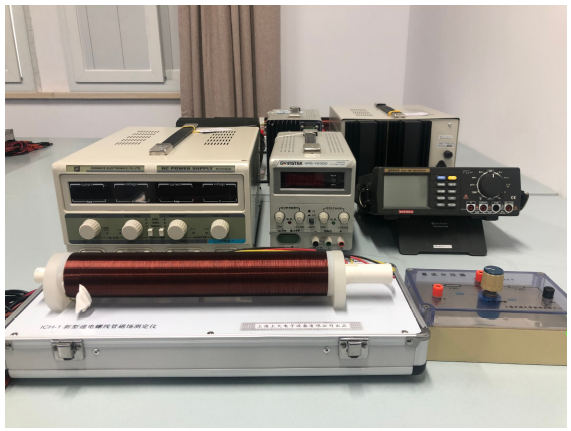
\includegraphics[scale = 0.6]{p3.png}
	\caption{Measurement setup.}
\end{figure}
\begin{figure}[H]
	\centering
	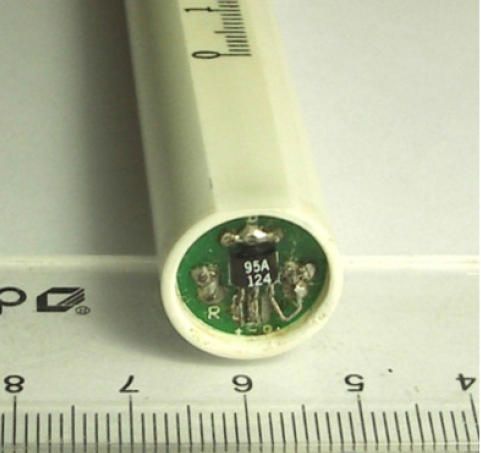
\includegraphics[scale = 0.6]{p4.png}
	\caption{Integrated Hall probe SS495A.}
\end{figure}

\subsection{Measurement Procedure}
\subsubsection{Relation Between Sensitivity $K_H$ and Working Voltage $U_S$}
First place the integrated Hall probe at the center of the solenoid(15 $cm$). 
Set the working voltage at 5V and measure the output voltage $U_0$(when $I_M = 0$) 
and $U$ (when $I_M = 250$ mA). Calculate the sensitivity of the probe $K_H$

Then Measure $K_H$ for different $U_S$ from 2.8V to 10V. Calculate $K_H/U_S$ and plot the 
curve $K_H/U_S$ vs $U_S$.

\subsubsection{Relation Between Output Voltage U and Magnetic Field B}
Set $B = 0$ and $U_S = 5$V, connect the 2.4 ~ 2.6 V output terminal of the DC voltage
divider and the negative port of the voltmeter, and adjust it until $U_0 = 0$. Then 
place the integrated Hall probe at the center of the solenoid(15 $cm$). Measure the output 
voltage $U$ for $I_M$ ranging from 0 to 500mA with intervals of 50 mA. Plot the curve $U$ vs. 
$B$ and find the sensitivity $K_H$.

\subsubsection{Magnetic Field Distribution Inside the Solenoid}
Set $I_M = 250$ mA, record the output voltage U with the position of the solenod $x$ varying. 


\section{Results}
The data sheet is attached to the end of this report.

The uncertainty calculation is included in the next part.
\subsection{Relation between Sensitivity $K_H$ and Working Voltage $U_S$}
The measurement data for U is in the following table:

\begin{table}[!h]
	\begin{center}
		\begin{tabular}{|c|c|c|}
			\hline
			$U_S$[V] & $U_0(I_M = 0)$[V]& $U(I_M = 250$mA)[V] \\ \hline
			5.00 & 2.517 & 2.636 \\ \hline
		\end{tabular}
		\caption{Data for $U_0$ and $U$ with $U_S$ = 5V}
	\end{center}
\end{table}

The uncertainties of these three data are:
\begin{table}[!h]
	\begin{center}
		\begin{tabular}{|c|c|c|}
			\hline
			$u_{U_S}$[V] & $u_{U_0}$[V]& $u_U$[V] \\ \hline
			0.03 & 0.007 & 0.007 \\ \hline
		\end{tabular}
		\caption{Uncertainties for $U_0$ and $U$ with $U_S$ = 5V}
	\end{center}
\end{table}

$K_H$ can be calculated by the following formula:
$$
K_H = \frac{U-U_0}{B} = \frac{2.636-2.517}{2.5\times1.4366\times10^{-3}} = 33.13 \pm 2.76V/T,\quad u_{K_{H},r} = 8.31\%
$$
  
We measured $K_H$ for different $U_S$ and calculated $K_H/U_S$ based on the following formula:
$$
\frac{K_H}{U_S} = \frac{U-U_0}{B\times U_S}
$$

The calculation results and scatter plot are listed below:
\begin{table}[H]
	\begin{center}
	\begin{tabular}{|l|l|l|l|l|}
	\hline
	   & $U_S$ & $u_{U_s}$ & $K_H/U_S$ & $u_{K_H/U_S}$ \\ \hline
	1  & 2.79  & 0.01      & 7.83      & 0.99          \\ \hline
	2  & 3.21  & 0.02      & 6.65      & 0.86          \\ \hline
	3  & 3.59  & 0.02      & 6.67      & 0.77          \\ \hline
	4  & 4.00  & 0.02      & 6.67      & 0.69          \\ \hline
	5  & 4.41  & 0.02      & 6.69      & 0.63          \\ \hline
	6  & 4.80  & 0.02      & 6.50      & 0.58          \\ \hline
	7  & 5.22  & 0.03      & 6.56      & 0.53          \\ \hline
	8  & 5.58  & 0.03      & 6.39      & 0.49          \\ \hline
	9  & 6.07  & 0.03      & 6.24      & 0.45          \\ \hline
	10 & 6.36  & 0.03      & 6.13      & 0.43          \\ \hline
	11 & 6.79  & 0.03      & 5.99      & 0.41          \\ \hline
	12 & 7.17  & 0.04      & 5.90      & 0.38          \\ \hline
	13 & 7.64  & 0.04      & 5.76      & 0.36          \\ \hline
	14 & 7.99  & 0.04      & 5.65      & 0.35          \\ \hline
	15 & 8.41  & 0.04      & 5.36      & 0.33          \\ \hline
	16 & 8.81  & 0.04      & 5.34      & 0.31          \\ \hline
	17 & 9.21  & 0.05      & 5.11      & 0.30          \\ \hline
	18 & 10.05 & 0.05      & 4.88      & 0.27          \\ \hline
	\end{tabular}
	\caption{Results for $K_H/U_S$}	
	\end{center}
\end{table}
	
\begin{figure}[H]
	\centering
	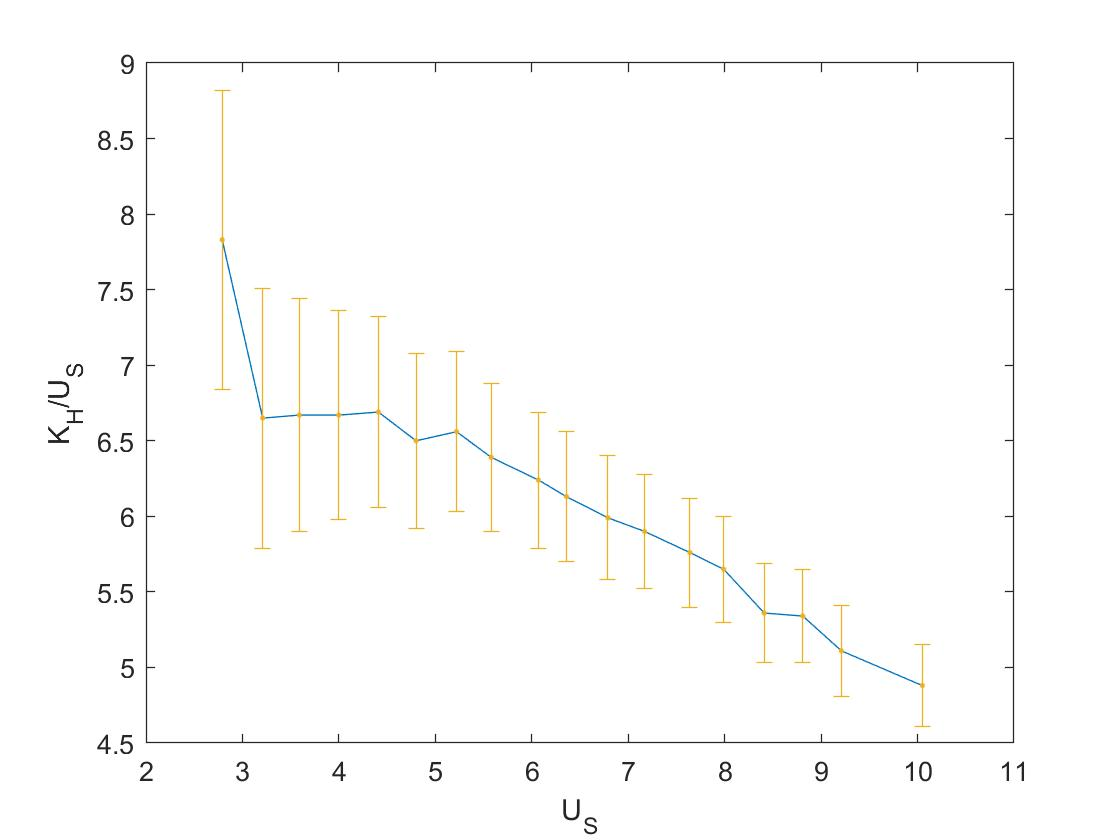
\includegraphics[scale = 0.3]{plot1.jpg}
	\caption{Scatter Plot for $K_H/U_S$ vs $U_S$}
\end{figure}

\subsection{Relation Between Output Voltage $U$ and Magnetic Field $B$}
The original data and its uncertainties are listed below:
\begin{table}[H]
	\begin{center}
		\begin{tabular}{|l|l|l|l|l|}
			\hline
			   & $I_M$[mA] & $U_A$[A] & $U$[mV]    & $u_U$[V]    \\ \hline
			1  & 0     & 0.000 & 0.00   & 0.000600 \\ \hline
			2  & 50    & 0.001 & 24.40  & 0.000612 \\ \hline
			3  & 100   & 0.002 & 49.22  & 0.000625 \\ \hline
			4  & 150   & 0.003 & 71.08  & 0.000636 \\ \hline
			5  & 200   & 0.004 & 94.42  & 0.000647 \\ \hline
			6  & 250   & 0.005 & 117.00 & 0.000659 \\ \hline
			7  & 300   & 0.006 & 140.86 & 0.000670 \\ \hline
			8  & 350   & 0.007 & 162.36 & 0.000681 \\ \hline
			9  & 400   & 0.008 & 184.90 & 0.000692 \\ \hline
			10 & 450   & 0.009 & 208.32 & 0.000704 \\ \hline
			11 & 500   & 0.010 & 232.4  & 0.000716 \\ \hline
			\end{tabular}
			\caption{Measurement data for $U$ vs $I_M$}
	\end{center}
\end{table}

Then we can calculate the magnitude of magnetic field for each electric current:
$$
B = \frac{U-U_0}{K_H} = \frac{U}{K_H}
$$

The calculation results and liner fit plot are listed below:
\begin{table}[H]
	\begin{center}
		\begin{tabular}{|l|l|l|l|l|}
			\hline
			   & $B${[}T{]} & $u_B[T]$ & $U${[}mV{]} & $u_U${[}V{]} \\ \hline
			1  & 0	        & 0.000000 & 0.00        & 0.000600     \\ \hline
			2  & 0.0007183  & 0.000015 & 24.40       & 0.000612     \\ \hline
			3  & 0.0014366  & 0.000030 & 49.22       & 0.000625     \\ \hline
			4  & 0.0021549  & 0.000045 & 71.08       & 0.000636     \\ \hline
			5  & 0.0028732  & 0.000059 & 94.42       & 0.000647     \\ \hline
			6  & 0.0035915  & 0.000074 & 117.00      & 0.000659     \\ \hline
			7  & 0.0043098  & 0.000089 & 140.86      & 0.000670     \\ \hline
			8  & 0.0050281  & 0.000104 & 162.36      & 0.000681     \\ \hline
			9  & 0.0057464  & 0.000119 & 184.90      & 0.000692     \\ \hline
			10 & 0.0064647  & 0.000134 & 208.32      & 0.000704     \\ \hline
			11 & 0.007183   & 0.000144 & 232.4       & 0.000716     \\ \hline
		\end{tabular}
		\caption{Results for U vs. B}
	\end{center}
\end{table}

\begin{figure}[H]
	\centering
	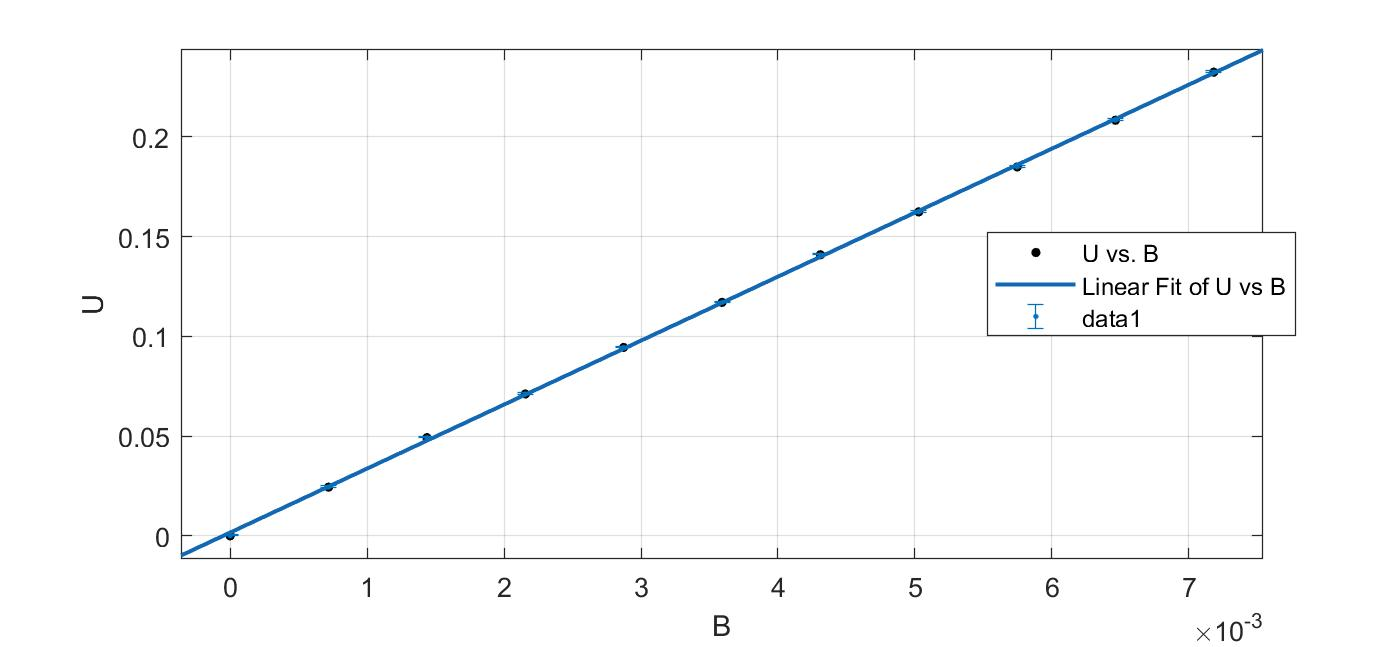
\includegraphics[scale = 0.3]{plot2.jpg}
	\caption{Linear Fit of U-B}
\end{figure}

Since $K_H = U/B$. We can read the sensitivity from the slope of the linear fit:
$$
K_H = 32.07\pm0.29V/T
$$

The deviation of experimental sensitivity form the theoretical value is:

\begin{align*}
	\Delta K &= \frac{K_{H,experimental} - K_{H_theory}}{K_{H_theory}} \times 100\%\\
			 &= \frac{32.07-33.13}{33.13} \times 100\%\\
			 &= -3.20\% 
\end{align*}

So we can see the experimental data is very close to the theoretical value, and the error is relativly small.

\subsection{Magnetic Field Distribution Inside the Solenoid}
In this section, we studied the magnetic field distribution inside the solenoid by measuring the corresponding
magnetic field. We can calculate the magnitude of magnetic field in relation to the distance. The results are listed 
in the tables below:

\begin{table}[H]
	\begin{center}
	\begin{tabular}{|l|l|l|l|l|l|l|l|}
	\hline
	   & $x${[}cm{]}$\pm 0.05${[}cm{]} & $U${[}mV{]} & $u_U${[}V{]} &    & $x${[}cm{]}$\pm 0.05${[}cm{]} & $U${[}mV{]} & $u_U${[}V{]} \\ \hline
	1  & 0.00                          & 13.20       & 0.000607     & 27 & 16.00                         & 118.21      & 0.000659     \\ \hline
	2  & 0.50                          & 19.15       & 0.000610     & 28 & 17.00                         & 118.07      & 0.000659     \\ \hline
	3  & 1.00                          & 27.79       & 0.000614     & 29 & 18.00                         & 117.85      & 0.000659     \\ \hline
	4  & 1.50                          & 39.30       & 0.000620     & 30 & 19.00                         & 117.38      & 0.000659     \\ \hline
	5  & 2.00                          & 55.13       & 0.000628     & 31 & 19.50                         & 117.19      & 0.000659     \\ \hline
	6  & 2.50                          & 73.88       & 0.000637     & 32 & 20.00                         & 117.08      & 0.000659     \\ \hline
	7  & 3.00                          & 86.60       & 0.000643     & 33 & 20.50                         & 116.98      & 0.000658     \\ \hline
	8  & 3.50                          & 96.53       & 0.000648     & 34 & 21.00                         & 116.78      & 0.000658     \\ \hline
	9  & 4.00                          & 102.50      & 0.000651     & 35 & 21.50                         & 116.50      & 0.000658     \\ \hline
	10 & 4.50                          & 107.11      & 0.000654     & 36 & 22.00                         & 116.27      & 0.000658     \\ \hline
	11 & 5.00                          & 110.03      & 0.000655     & 37 & 22.50                         & 115.90      & 0.000658     \\ \hline
	12 & 5.50                          & 112.20      & 0.000656     & 38 & 23.00                         & 115.36      & 0.000658     \\ \hline
	13 & 6.00                          & 113.71      & 0.000657     & 39 & 23.50                         & 114.51      & 0.000657     \\ \hline
	14 & 6.50                          & 114.68      & 0.000657     & 40 & 24.00                         & 113.29      & 0.000657     \\ \hline
	15 & 7.00                          & 115.42      & 0.000658     & 41 & 24.50                         & 112.15      & 0.000656     \\ \hline
	16 & 7.50                          & 116.06      & 0.000658     & 42 & 25.00                         & 110.20      & 0.000655     \\ \hline
	17 & 8.00                          & 116.53      & 0.000658     & 43 & 25.50                         & 107.61      & 0.000654     \\ \hline
	18 & 8.50                          & 117.09      & 0.000659     & 44 & 26.00                         & 103.71      & 0.000652     \\ \hline
	19 & 9.00                          & 117.31      & 0.000659     & 45 & 26.50                         & 97.55       & 0.000649     \\ \hline
	20 & 9.50                          & 117.44      & 0.000659     & 46 & 27.00                         & 89.20       & 0.000645     \\ \hline
	21 & 10.00                         & 117.54      & 0.000659     & 47 & 27.50                         & 75.34       & 0.000638     \\ \hline
	22 & 11.00                         & 117.61      & 0.000659     & 48 & 28.00                         & 62.15       & 0.000631     \\ \hline
	23 & 12.00                         & 117.70      & 0.000659     & 49 & 28.50                         & 43.60       & 0.000622     \\ \hline
	24 & 13.00                         & 117.90      & 0.000659     & 50 & 29.00                         & 30.38       & 0.000615     \\ \hline
	25 & 14.00                         & 118.11      & 0.000659     & 51 & 29.50                         & 20.55       & 0.000610     \\ \hline
	26 & 15.00                         & 118.20      & 0.000659     & 52 & 30.00                         & 14.94       & 0.000607     \\ \hline
	\end{tabular}
	\caption{Measurement data for the distribution of magnetic field}		
	\end{center}
\end{table}

\begin{table}[H]
	\begin{center}
	\begin{tabular}{|l|l|l|l|l|l|l|l|}
	\hline
	   & $x${[}cm{]}$\pm 0.05${[}cm{]} & B(x){[}T{]} & $u_B${[}T{]} &    & $x${[}cm{]}$\pm 0.05${[}cm{]} & B(x){[}T{]} & $u_B${[}T{]} \\ \hline
	1  & 0.00                          & 0.000398430 & 0.00004      & 27 & 16.00                         & 0.003568065 & 0.00030      \\ \hline
	2  & 0.50                          & 0.000578026 & 0.00005      & 28 & 17.00                         & 0.003563839 & 0.00030      \\ \hline
	3  & 1.00                          & 0.000838817 & 0.00007      & 29 & 18.00                         & 0.003557199 & 0.00030      \\ \hline
	4  & 1.50                          & 0.001186236 & 0.00010      & 30 & 19.00                         & 0.003543012 & 0.00030      \\ \hline
	5  & 2.00                          & 0.001664051 & 0.00014      & 31 & 19.50                         & 0.003537277 & 0.00030      \\ \hline
	6  & 2.50                          & 0.002230003 & 0.00019      & 32 & 20.00                         & 0.003533957 & 0.00030      \\ \hline
	7  & 3.00                          & 0.002613945 & 0.00022      & 33 & 20.50                         & 0.003530939 & 0.00029      \\ \hline
	8  & 3.50                          & 0.002913673 & 0.00024      & 34 & 21.00                         & 0.003524902 & 0.00029      \\ \hline
	9  & 4.00                          & 0.003093873 & 0.00026      & 35 & 21.50                         & 0.003516450 & 0.00029      \\ \hline
	10 & 4.50                          & 0.003233021 & 0.00027      & 36 & 22.00                         & 0.003509508 & 0.00029      \\ \hline
	11 & 5.00                          & 0.003321159 & 0.00028      & 37 & 22.50                         & 0.003498340 & 0.00029      \\ \hline
	12 & 5.50                          & 0.003386659 & 0.00028      & 38 & 23.00                         & 0.003482040 & 0.00029      \\ \hline
	13 & 6.00                          & 0.003432237 & 0.00029      & 39 & 23.50                         & 0.003456384 & 0.00029      \\ \hline
	14 & 6.50                          & 0.003461515 & 0.00029      & 40 & 24.00                         & 0.003419559 & 0.00029      \\ \hline
	15 & 7.00                          & 0.003483851 & 0.00029      & 41 & 24.50                         & 0.003385149 & 0.00028      \\ \hline
	16 & 7.50                          & 0.003503169 & 0.00029      & 42 & 25.00                         & 0.003326290 & 0.00028      \\ \hline
	17 & 8.00                          & 0.003517356 & 0.00029      & 43 & 25.50                         & 0.003248113 & 0.00027      \\ \hline
	18 & 8.50                          & 0.003534259 & 0.00030      & 44 & 26.00                         & 0.003130395 & 0.00026      \\ \hline
	19 & 9.00                          & 0.003540899 & 0.00030      & 45 & 26.50                         & 0.002944461 & 0.00025      \\ \hline
	20 & 9.50                          & 0.003544823 & 0.00030      & 46 & 27.00                         & 0.002692424 & 0.00023      \\ \hline
	21 & 10.00                         & 0.003547842 & 0.00030      & 47 & 27.50                         & 0.002274072 & 0.00019      \\ \hline
	22 & 11.00                         & 0.003549955 & 0.00030      & 48 & 28.00                         & 0.001875943 & 0.00016      \\ \hline
	23 & 12.00                         & 0.003552671 & 0.00030      & 49 & 28.50                         & 0.001316028 & 0.00011      \\ \hline
	24 & 13.00                         & 0.003558708 & 0.00030      & 50 & 29.00                         & 0.000916994 & 0.00008      \\ \hline
	25 & 14.00                         & 0.003565047 & 0.00030      & 51 & 29.50                         & 0.000620284 & 0.00005      \\ \hline
	26 & 15.00                         & 0.003567763 & 0.00030      & 52 & 30.00                         & 0.000450951 & 0.00004      \\ \hline
	\end{tabular}
	\caption{Data for distribution of magnetic field}		
	\end{center}
\end{table}

Since $I_M = 250mA$, we can derive that $B_{theoretical}$ = 2.5$B_{0.1}(x)$.

The calculation results are shown below:
\begin{table}[H]
	\begin{center}
	\begin{tabular}{|l|l|l|l|}
	\hline
	$x${[}m{]} & $B_{theo}${[}T{]} & $x${[}m{]} & $B_{theo}${[}T{]} \\ \hline
	$\pm$0.000 & 0.0035915         & $\pm$0.080 & 0.0035143         \\ \hline
	$\pm$0.010 & 0.0035908         & $\pm$0.090 & 0.0034640         \\ \hline
	$\pm$0.020 & 0.0035890         & $\pm$0.100 & 0.0033695         \\ \hline
	$\pm$0.030 & 0.0035858         & $\pm$0.110 & 0.0031713         \\ \hline
	$\pm$0.040 & 0.0035808         & $\pm$0.120 & 0.0029908         \\ \hline
	$\pm$0.050 & 0.0035730         & $\pm$0.130 & 0.0027158         \\ \hline
	$\pm$0.060 & 0.0035613         & $\pm$0.140 & 0.0023153         \\ \hline
	$\pm$0.070 & 0.0035433         & $\pm$0.150 & 0.0018083         \\ \hline
	\end{tabular}
	\caption{Theoretical value of the magnetic field inside the solenoid($I_M = 250mA$)}
	\end{center}
\end{table}

Finally we can plot the scatter plot of $B$ vs. $x$:
\begin{figure}[H]
	\centering
	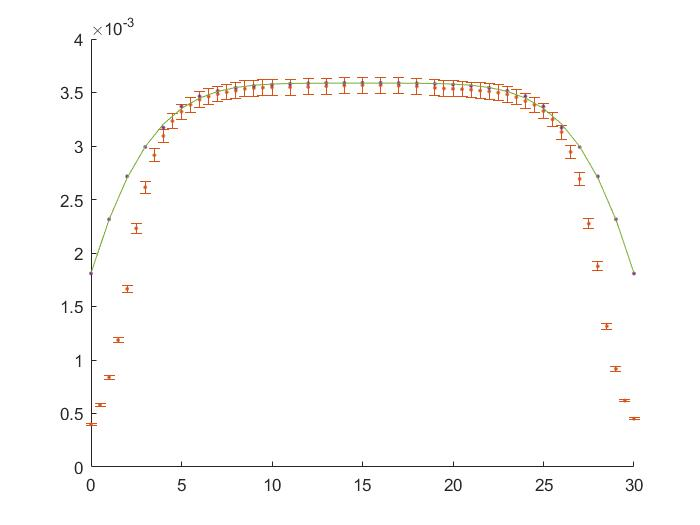
\includegraphics[scale = 0.4]{plot3.jpg}
	\caption{The magnetic field in side the solenoid($I_M$ = 250mA).}
\end{figure}



\section{Uncertainty analysis}
\subsection{Relation between Sensitivity $K_H$ and Working Voltage $U_S$}
The uncertainties of $U_0(I_M = 0[V])$ and $U_0(I_M = 250mA)[V]$ can be calculated as:
\begin{align*}
	u_{U_S} = 5.00 \times 0.5\% &= 0.03V
	\\
	u_{U_0} = 2.517 \times 0.05\% + 6 \times 10^{-3} &= 0.007V
	\\
	u_U = 2.636 \times 0.05\% + 6 \times 10^{-3} &= 0.007V	
\end{align*}

Then the uncertainty for $K_H$ can be calculated by the equation $K_H=\frac{U-U_0}{B}$ as:
\begin{align*}
	u_{K_H}&=\sqrt{\left(\frac{\partial K_H}{\partial U}\right)^2u_U^2+\left(\frac{\partial K_H}{\partial U_0}\right)^2u_{U_0}^2}\\
	&=\left(\frac{1}{B}\right)\times\sqrt{u_U^2+u_{U_0}^2}\\
	&=2.76\,\rm{V/T}\\
	u_{K_{H},r} &=8.31\% 
\end{align*}
So that $K_H = 33.13\pm2.76V/T, \quad u_{K_H,r} = 8.3\%$

The uncertainty of $K_H/U_S$ can be calculated by the formula $K_H/U_S = (U-U_0)/(B\times U_S)$:
\begin{align*}
	u_{K_H/U_S}&=\sqrt{\left(\frac{\partial K_H/U_S}{\partial K_H}\right)^2u_{K_H}^2+\left(\frac{\partial K_H/U_S}{\partial U_S}\right)^2u_{U_S}^2}\\
	&=\sqrt{\left(\frac{1}{U_S}\right)^2u_{K_H}^2+\left(\frac{1}{U_S^2}\right)^2u_{U_S}^2}\\
\end{align*}
When $U_S = 2.79V$, $u_{K_H/U_S}$ can be calculated as:
\begin{align*}
	u_{K_H/U_S} &= \sqrt{(1/2.79)^2 \times (2.76)^2 + (1/2.79^2)^2 \times 0.01^2}\\
				&= 0.99 T^{-1}
\end{align*}

\subsection{Relation Between Output Voltage $U$ and Magnetic Field $B$}
The uncertainty for $I_M$ can be calclated as:
$$
u_{I_M} = I_M \times 2\%
$$

When $I_M = 500mA$:
$$
u_{I_M} = 500mA \times 2\% = 0.01A
$$

The uncertainty for $U$ can be calculated as:
$$
u_U = U \times 0.05\% + 6\times 10^{-4}
$$

When $U = 232.4 mV$:
$$
u_U = 232.4 \times 0.05\% + 6 \times 10^{-4} = 0.000117V
$$

The uncertainty for $B_{I_M}$ can be calclated as:
$$
u_B = \frac{B_{0.1A}}{0.1} \times u_{I_M}
$$

When $I_M = 500 mA$:
$$
u_B = \frac{1.4366}{0.1}\times 0.01 = 0.000144
$$

\subsection{Magnetic Field Distribution Inside the Solenoid}
We have already found the uncertainty of U:
$$
u_U = U\times 0.05\% + 6\times 10^{-4}
$$

The uncertanty of $B(x)$ can be calculated as:
\begin{align*}
	u_B &= \sqrt{\left( \frac{\partial B}{\partial U}u_U \right)^2 + \left( \frac{\partial B}{\partial K_H}u_{K_H} \right)^2 }
	\\  &= \sqrt{\left(\frac{u_U}{K_H}\right)^2 + \left( - \frac{U}{K_H^2}u_{K_H}\right)^2}
\end{align*}

When $x = 0.00 cm$:
$$
u_B = \sqrt{(0.000607/33.12)^2+(0.01320\times2.76/33.12^2)^2} = 0.00004
$$

\section{Conclusion and discussion}
In this lab we studied the principle of Hall effect and its applications using a Hall probe. It 
is used to verify that the Hall voltage is proportional to the magnetic field. The sensitivity of 
an integrated Hall probe is studied by calculating the magnetic field at the center of the solenoid, 
and the magnetic field distribution along the axis of the solenoid is measuerd and compared with 
the theoretical value.

The experimental errors mainly come from the experimental apparatuses. Since the numbers on the equipments 
are changing constantly, it's very hard to find a stable and reliable data to record. On most cases I have to 
estimate the value so that the result is very inaccurate. If only the equipments are more accurate or if it can 
evaluate the mean value for me, I can make the result more accurate.

Also since the magnetic field generated in the Hall Probe is quite small, the magnetic field of the Earth can not 
be ignored.

In the experiment \textbf{Relation Between Sensitivity $K_H$ and Working Voltage $U_S$}, We find the $K_H$ with 
respect to $U_S$ and plot the scatter graph. We then find that when $U_S = 5V$, $K_H$ is most stable, so we choose 
5V as the working voltage in the following experiments.

In the experiment \textbf{Relation Between Output Voltage U and Magnetic Field B}, we find the relation between Hall 
voltage $U_H$ and the magnetic field $B$. According to the linear fit, we can see that $U_H$ and $B$ has a linear relationship, 
which fits the theory. The experimental value $K_H$ can be read from the slope of liner fit as 32.07$\pm$0.29 V/T. The 
deviation of experimental value from theoretical value is -3.20\%, which is relativly small and proves the theory.

In the experiment \textbf{Magnetic Field Distribution Inside the Solenoid}, we measured the magnetic field at different places along 
the solenoid. We can find that the magnetic field is strongest in the middle of the solenoid, and it decreses quickly when it goes 
far from the middle. Then we plot the experimental and theoretical on the same graph, and we can find them fit well.




\section{References}
    \begin{enumerate}
        \item Qin Tian, Cao Jianjun, Yi Hankun, Wu Ziyou, Zhang Yifei, Yao Yuan, Mateusz Krzyzosiak
    \end{enumerate}

\end{document}
